% English r27, synchronized to Chinese r27. Compile with pdfLaTeX.
\documentclass[conference,10pt,letterpaper]{IEEEtran}
\usepackage[T1]{fontenc}
\usepackage[utf8]{inputenc}
\usepackage{courier}
\usepackage{graphicx,booktabs,tabularx,array,url,amsmath,microtype}
\usepackage[hidelinks]{hyperref}
\newcolumntype{Y}{>{\raggedright\arraybackslash}X}
\newcolumntype{P}[1]{>{\raggedright\arraybackslash}p{#1}}
\setlength{\emergencystretch}{1.5em}
\setlength{\textfloatsep}{12pt plus 2pt minus 2pt}
\setlength{\dbltextfloatsep}{12pt plus 2pt minus 2pt}
\setlength{\floatsep}{10pt plus 2pt minus 2pt}
\setlength{\dblfloatsep}{10pt plus 2pt minus 2pt}
\renewcommand{\topfraction}{0.9}
\renewcommand{\bottomfraction}{0.85}
\renewcommand{\textfraction}{0.1}
\renewcommand{\floatpagefraction}{0.8}
\renewcommand{\dbltopfraction}{0.9}
\renewcommand{\dblfloatpagefraction}{0.8}
\setcounter{topnumber}{3}
\setcounter{bottomnumber}{2}
\setcounter{totalnumber}{4}
\setcounter{dbltopnumber}{3}
\makeatletter
\setlength{\@fptop}{0pt}
\setlength{\@fpsep}{12pt}
\setlength{\@fpbot}{0pt plus 1fil}
\makeatother
\hypersetup{pdftitle={Z-ParaPack: Packing File Updates and Parallelizing Appends on ZNS SSDs},pdfauthor={Anonymous Authors}}
\title{Z-ParaPack: Packing File Updates and Parallelizing Appends on ZNS SSDs}
\author{\IEEEauthorblockN{Anonymous Authors}}
\begin{document}
\maketitle
\pagestyle{plain}
\thispagestyle{plain}
\begin{abstract}
Synchronous updates to independent files still contend for a few shared append states inside the filesystem.
On Zoned Namespace (ZNS) solid-state drives (SSDs), distributing appends must respect active and open zone limits while preserving synchronization semantics for all pending mappings.
These mappings include obligations from earlier asynchronous writeback, even after the corresponding data pages become clean.

Z-ParaPack organizes file-update commit closures together with append permissions.
An update pack (PACK) gathers current writeback and pending mappings; a terminal record in the last selected node defines durable completion.
Reusable append lanes separate allocation state across concurrent updates and reserve a lane for maintenance writes.
Recovery validates and replays complete PACKs in commit-number order.
On Linux 7.2.9, Z-ParaPack exceeds the fastest baseline under highly concurrent synchronous random writes and increases completion rates for mixed file operations, database transactions, and persistent messaging.
Both SQLite configurations improve transaction completion rates and achieve the lowest p99.9 among the evaluated systems.
Path analysis shows shorter shared-allocation intervals together with shorter complete synchronization calls at high concurrency.
\end{abstract}
\begin{IEEEkeywords}
ZNS SSD, file systems, file synchronization, parallel append, crash recovery.
\end{IEEEkeywords}

\section{Introduction}\label{sec:introduction}
SQLite clients updating independent databases and NATS JetStream connections publishing to different streams must wait for durable completion before processing subsequent requests.
Although these updates have no data dependencies across files, the filesystem can make them compete for the same append position.
As concurrency increases, shared allocation state becomes a serialization point on the application's persistence path.

Zoned Namespace (ZNS) solid-state drives (SSDs) delegate append-state management to the host.
The host appends sequentially within zones and respects limits on active and open zones~\cite{r3,r5,r9}.
Open zones permit appends; active zones also include closed zones that have yet to finish.
Concurrent file updates, background writeback, checkpoints, and garbage collection (GC) must share these finite append resources.

F2FS organizes logs by data pages (DATA), node pages (NODE), and temperature class.
Each class shares current-segment state (curseg), with a mutex protecting the next append position~\cite{r1}.
ScaleLFS improves GC parallelism, and Z-LFS manages ZNS log resources~\cite{r5,r8}.
Their public code and our Linux 7.2 ports still select curseg by block type for ordinary writeback~\cite{r13,r14}.
Adding GC streams or increasing the zones available to logs leaves ordinary updates of the same class sharing an allocation entry point.
In our Linux 7.2.9 experiment with 64\,KiB writes followed by synchronization, F2FS, ScaleLFS, and Z-LFS throughput declines beyond four threads.
At 32 threads, F2FS DATA/NODE curseg intervals occupy 93.9\% of the full sampled \texttt{fsync} call.

Separating append state by file update also requires a commit boundary that preserves synchronization semantics.
Each \texttt{fsync} must confirm current DATA writeback and mappings from earlier asynchronous writeback.
Those earlier mappings remain pending even after their DATA pages become clean.
We call the mappings and related nodes that one synchronization must confirm its \emph{commit closure}.
Distributing DATA alone retains the shared NODE allocation entry point.
After distributing NODEs as well, synchronization must identify its completed commit record, and recovery must distinguish updates whose appends interleave.

Prior work provides foundations for parallel logs and synchronization ordering.
Max dynamically assigns complete file operations to log partitions and merges recovery through global versions~\cite{r2}.
ScaleZNFS adds hot/warm DATA logs, per-log scheduling, and ZNS-driven ordered completion while retaining one log per NODE type and F2FS recovery~\cite{r3}.
Z-ParaPack addresses commit semantics after distributing DATA and related NODEs within finite zone resources.
It combines mapping closures across writeback batches, confirmation of the completed commit, and recovery order in one file-update protocol.

Z-ParaPack represents a commit closure with an update pack (PACK) and manages append permission through leased append lanes.
A PACK appends its current DATA and selected NODEs to its leased lane.
The last selected NODE carries the commit record, called the \emph{terminal}.
Synchronization waits for that terminal and checks errors; recovery validates the terminal and node chain, then replays complete updates in commit-number order.
Ordinary non-inline DATA writeback shares file-update lanes with PACKs.
A reserved maintenance lane carries NODEs outside commits, directories, and GC writes.
Commits and asynchronous batches reuse lanes under common physical active/open limits.

\begin{figure*}[t]\centering
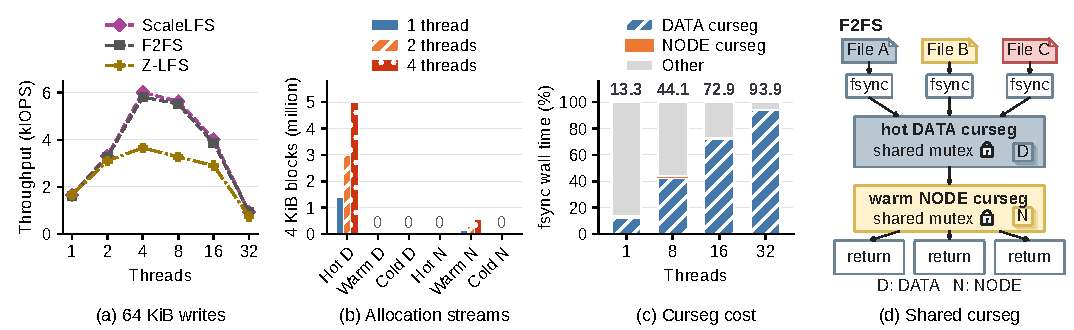
\includegraphics[width=\textwidth]{./figures/compact_motivation64k.pdf}
\caption{Shared allocation with 64\,KiB synchronous updates. (a) Baseline throughput scaling; (b) block counts for six F2FS allocation streams; (c) DATA/NODE curseg intervals within full sampled fsync calls, with combined percentages above bars; (d) schematic of files sharing curseg. D/N denote DATA/NODE in (b). Each numerical panel uses its own measurement protocol.}\label{fig:motivation}
\end{figure*}

Our contributions are:
\begin{enumerate}
\item PACK combines commit closures with parallel appends.
It gathers current writeback and pending mappings, using related NODEs and a terminal to define recoverable updates.
Lanes separate allocation state across updates and support ordered recovery of interleaved commits.
\item Separate append state supports commits and maintenance within finite zone resources.
Leases grant append permission, while a shared physical ledger accounts for active/open occupancy.
Commits return permission before maintenance that may depend on checkpoints or GC; maintenance uses its reserved lane.
\item The implementation increases durable completion rates and reduces extreme tail latency.
On Linux 7.2.9, 4\,KiB synchronous random writes at 32 threads reach 41.27\,kIOPS, 5.58$\times$ F2FS, the fastest baseline under that condition.
With sixteen SQLite databases, transaction throughput reaches 1.94$\times$ the fastest baseline, F2FS, while p99.9 falls 73.4\% below Btrfs, the lowest-latency baseline.
FileMicro synchronous writes and NATS publishes reach about 1.9$\times$ their fastest baselines; extended Varmail also improves mixed file operations.
\end{enumerate}

\section{Background and Motivation}\label{sec:motivation}
\subsection{Independent Durable Updates and Finite Append Resources}
Independent file updates provide opportunities for parallel persistence.
Different databases and message streams update their own files, and \texttt{fsync} must confirm each file's contents and recovery metadata.
The filesystem must still allocate new blocks for overwrites, update mappings, and return after durable completion.

ZNS requires sequential appends within each zone and separately limits active and open zones.
Closing a partially written zone releases open occupancy but retains active occupancy.
Our device permits sixteen of each, so 32 workers cannot obtain 32 physical append heads by permanently reserving one writable zone each.
Software request concurrency and physical zone occupancy therefore require separate management.
Foreground commits, ordinary asynchronous writeback, and GC must share this budget.

\subsection{Independent Updates Converge on Shared Allocation State}
F2FS stores file contents in DATA and inode information and block addresses in NODE~\cite{r1}.
An overwrite allocates a new DATA location and records its address in the corresponding NODE.
Both block types occupy the main area (MAIN).
The six-log configuration selects curseg by DATA/NODE and hot, warm, or cold class.
Each curseg records a segment number, summary, and next allocation position.
Files in the same class acquire the same curseg mutex to allocate addresses, record summaries, and advance offsets.

ScaleLFS adds independent GC streams, and Z-LFS expands the zones available to logs.
Ordinary file writeback in both systems retains type-based curseg sharing~\cite{r5,r8,r13,r14}.
Adding reclamation streams or available zones addresses a different layer of concurrency from separating ordinary updates' allocation state.

Files that update independently at the application converge on the same curseg in the allocator.
Figure~\ref{fig:motivation} examines this sharing through throughput, allocation streams, and synchronization paths.
All numerical panels use 64\,KiB updates, with separate runs for throughput, allocation counts, and path diagnostics.
Section~\ref{sec:cost} defines the diagnostic protocols.



As concurrency increases, completion rates for all three baselines rise and then decline.
F2FS, ScaleLFS, and Z-LFS peak at four threads in Figure~\ref{fig:motivation}(a), at 5.82, 6.02, and 3.66\,kIOPS, respectively.
At 32 threads, their rates fall to 0.93, 0.93, and 0.75\,kIOPS.
F2FS allocation counts locate the sharing across files.
At one, two, and four threads, all DATA enters hot DATA and all NODEs enter warm NODE, while the other four streams receive zero blocks (Figure~\ref{fig:motivation}(b)).
Different files thus access the same DATA or NODE allocation state (Figure~\ref{fig:motivation}(d)).

This sharing also appears within complete synchronization calls.
DATA/NODE curseg acquisition and hold intervals occupy 13.3\% of sampled \texttt{fsync} time at one thread, rising to 44.1\%, 72.9\%, and 93.9\% at eight, sixteen, and 32 threads.
At 32 threads, the complete call takes 40.845\,ms, including 38.369\,ms across the two curseg classes.
Acquisition intervals include execution, queuing, and scheduling; Other covers remaining synchronization work and \texttt{balance}.
These measurements locate elapsed time on the shared allocation path.

\subsection{Jointly Organizing Parallel Allocation and Recoverable Commits}\label{sec:joint}
The observations expose different organizational units at the application and allocator.
Applications update independent files, while allocation shares state across a few log classes.
Separating append state by concurrent file update can reduce contention at those entry points.
ZNS limits and file synchronization semantics further determine how these states can operate.

Software append lanes must reuse finite physical resources.
Each commit or asynchronous writeback batch acquires and releases append permission so subsequent updates can reuse the lane.
Maintenance uses a reserved lane under the same physical zone limits.
Partitioning software state by core or thread still requires common accounting for active/open occupancy.

Mapping obligations can also outlive an append lease.
Suppose asynchronous writeback overwrites block $a$ of an existing file at $a'$, clears the DATA dirty flag, and releases the old lease.
The application then overwrites block $b$ and calls \texttt{fsync}.
This synchronization must confirm mappings for both $a'$ and the newly written $b'$.
Inspecting current dirty DATA pages misses $a'$; adding DATA logs alone leaves the corresponding NODEs sharing an allocation entry point.
After distributing NODEs, the original fsync-node sequence no longer directly identifies this commit's terminal.
Physical scan order across lanes also cannot determine commit order.
The commit protocol must connect mapping obligations across leases to selected NODEs and the terminal that confirms them.

Z-ParaPack uses PACK to define each update's commit closure and lanes to separate append state across updates.
Leases manage append permission within the common zone budget.
Terminals and commit numbers identify complete PACKs and their recovery order, while a reserved maintenance lane carries writeback and reclamation outside commits.

\section{Z-ParaPack Design}\label{sec:design}
\subsection{PACKs and Lanes Organize Parallel File Updates}\label{sec:overview}
A PACK defines the contents that one synchronization must make durable; a lane manages the append permission needed to write those contents.
Z-ParaPack retains F2FS file mappings and block-validity semantics and gathers current writeback and pending mappings into each PACK.
The PACK appends current DATA and selected NODEs to its leased lane, with a terminal in the last selected NODE confirming completion.
Recovery validates and replays complete updates within the corresponding checkpoint generation.
Files have no permanent lane binding; subsequent updates can reuse lanes after lease release.

The system uses fifteen file-update lanes and one maintenance lane.
Ordinary non-inline DATA writeback uses file-update lanes by batch; \texttt{fsync}, \texttt{fdatasync}, and synchronous writes organize PACKs on these lanes.
A PACK's current DATA and related NODEs share its lane, although its closure can reference DATA from earlier writes on other lanes.
The maintenance lane handles NODEs outside commits, directories, quotas, and GC writes.

Figure~\ref{fig:architecture} traces parallel file updates through owners, lanes, and completion confirmation.
An owner coordinates synchronization; shared protection shards for the Segment Information Table (SIT) protect block validity.
Figure~\ref{fig:closure} expands closure selection and terminal confirmation for one PACK.
Figures~\ref{fig:lease} and~\ref{fig:recovery} explain append-permission reuse and commit recovery.

\begin{figure}[t]\centering
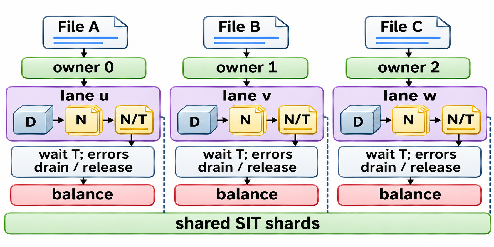
\includegraphics[width=.94\columnwidth]{./figures/redraw_architecture.pdf}
\caption{Independent files append DATA (D) and NODEs (N) through separate lanes, confirm the terminal (T) in the last NODE, drain, release leases, and run balance. Owners coordinate synchronization; dashed lines denote shared SIT protection. Files have no permanent lane binding.}\label{fig:architecture}
\end{figure}

\subsection{Mapping Closures Cover Updates Across Leases}\label{sec:closure}
Figure~\ref{fig:closure}(a) follows the $a'$, $b'$ example in Section~\ref{sec:joint}.
Earlier asynchronous writeback has written $a'$ and released its lease, but the mapping still awaits confirmation.
The current PACK includes this obligation together with the mapping obligation from writing $b'$.
It retains the NODE contents and marks that F2FS synchronization and roll-forward recovery require~\cite{r1}.

Mapping updates accumulate pending node identifiers (NIDs).
Synchronization first submits current DATA and records the corresponding NIDs (step~1), then captures the pending set and mapping-change sequence.
It adds the captured NIDs to the selection set (step~2).
The pending set can contain obligations from both earlier mappings and current writeback.
After waiting for the required DATA, the path deduplicates by NID and freezes the selection (step~3).
Per-inode pending and selection arrays grow as needed.
NIDs $a$, $b$ and their NODEs illustrate the process; updates can involve different numbers of nodes.

The path locks the entire selected NODE set and rechecks page identities, checkpoint generation, and mapping-change sequence (step~4).
Publishing a new mapping advances the sequence.
If this recheck detects a sequence change, the path abandons the PACK and falls back to a checkpoint as its dependencies require.
A stable selection enters the NODE append suffix in Figure~\ref{fig:closure}(b).
The DATA at $a'$ stays in place; current NODE writes confirm its mapping.
After a successful commit, the path clears pending entries only if the generation and sequence still match the snapshot, preserving obligations from later updates.

\begin{figure*}[t]\centering
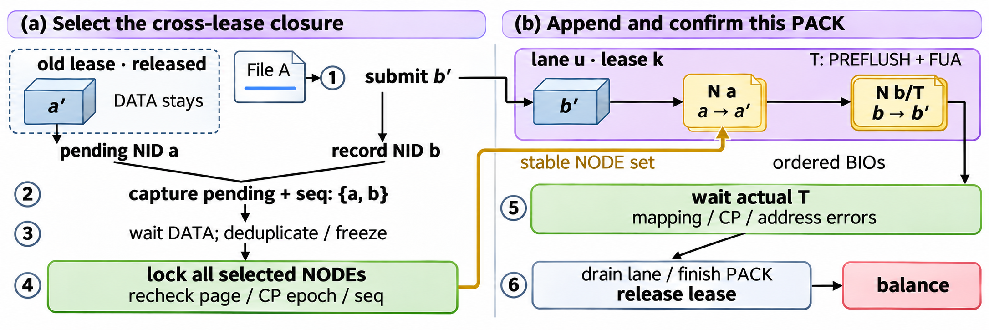
\includegraphics[width=.92\textwidth]{./figures/redraw_closure_terminal.pdf}
\caption{Cross-lease mapping closure and current commit. (a) Steps 1--4 submit current DATA, capture pending NIDs and sequence, wait and freeze a deduplicated selection, then recheck under locks. (b) Current $b'$ and selected NODEs share a lane; the last NODE carries T. Step~5 checks the actual T and errors; step~6 drains and releases the lease before balance. Earlier $a'$ stays in place; NIDs and node counts are illustrative.}\label{fig:closure}
\end{figure*}

\subsection{The Actual Terminal Defines Durable Completion}\label{sec:terminal}
Completion after distributing NODEs must refer to the current PACK.
The original fsync-node wait processes a list prefix by filesystem-wide node sequence number.
That prefix can include NODEs on other lanes, and the wait does not verify this PACK's terminal address.
Z-ParaPack tracks the page and block address of the last selected NODE and waits for that terminal.
This removes the wait point's dependency on NODEs from other lanes.
PACK NODEs retain node semantics; the block layer writes them to the lane through DATA-class block I/O units (BIOs).

In Figure~\ref{fig:closure}(b), current DATA $b'$ shares the lane with the selected NODEs.
N~a records the mapping for earlier DATA $a'$, while N~b/T records the mapping for $b'$ and carries the terminal.
On-disk next addresses connect the selected NODEs.
The last NODE uses that field for commit identity and a checksum.

The lane's ordered queue submits each BIO after its predecessor completes.
Current DATA and preceding NODEs use ordinary write requests.
The terminal requests a preflush (PREFLUSH) and force unit access (FUA).
When the device honors FLUSH/FUA semantics, terminal completion establishes durability for current DATA and selected NODEs.
It also confirms the closure's mappings for DATA from earlier asynchronous writeback.

Error handling follows the same completion boundary.
The queue records the first I/O error and completes subsequent requests with an error.
After the terminal page finishes writeback, synchronization also checks DATA/NODE mapping errors, checkpoint errors, and the terminal's submitted address.
Any failed check returns an error.
If an error follows submission of a NODE prefix, the path stops subsequent commits so that the prefix cannot connect to the next PACK's terminal.

After checking the terminal and errors (step~5), the path ends the PACK and waits for lane drainage.
Drain errors also affect the return status.
It then releases the lease (step~6), runs \texttt{balance}, and returns to the caller.
If the path cannot form a stable closure or acquire resources, it releases append protection and completes through a checkpoint as dependencies require.
The inode page and dentry recovery marks can cover inline DATA.
For eligible new small, empty, or inline files, the inode page can carry the terminal.
New files first exceeding inode coverage, and operations requiring global recovery metadata, use a checkpoint.



\subsection{Reusable Permissions Share a Physical Zone Ledger}\label{sec:lease}
Software lane reuse and physical zone release have different boundaries.
A lease identifies a lane and generation; allocation verifies permission before publishing an address.
After lease release, another update can use the lane.
Written zones can still occupy active or open resources, so foreground commits, asynchronous writeback, and maintenance share a physical ledger.
For each resource, the ledger maintains accounted occupancy plus reserved new occupancy within the device limit.

Physical operations reserve new occupancy before issuing device commands.
In Figure~\ref{fig:lease}, closing a partially written zone releases only open occupancy.
Successful finish or reset operations update the corresponding credits according to the resulting state.
GC relocation still coordinates with checkpoints, in-flight I/O, and read references; a failed operation cannot directly yield reusable credits.
Lease release returns software append permission without changing physical occupancy.

Commits and asynchronous batches release leases before entering maintenance that may depend on checkpoints or GC.
Subsequent file updates can therefore reuse their append state.
NODEs outside commits, directories, quotas, and GC writes use the reserved maintenance lane, leaving file-update append entry points available.
Both lane classes obey common physical limits; the maintenance lane adds no active or open capacity.

\begin{figure}[t]\centering
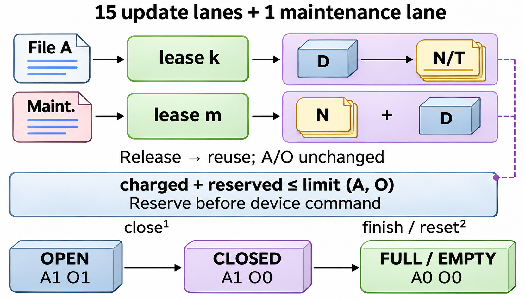
\includegraphics[width=\columnwidth]{./figures/redraw_lease_budget.pdf}
\caption{Lease release permits lane reuse; zone state determines physical occupancy. All lanes share active (A)/open (O) accounting and reserve new occupancy first. States follow successful operations: closing a partially written zone releases O; finish/reset updates A/O by resulting state. Dashed lines denote accounting. Lease and checkpoint generations remain separate.}\label{fig:lease}
\end{figure}

\subsection{Checkpoint Generations Scope Ordered Recovery}\label{sec:recovery}
Physical positions locate nodes after distributed appends; commit numbers determine replay order.
A checkpoint records the lane layout and on-disk recovery descriptors.
Within each generation, PACKs obtain globally ordered commit numbers from a shared sequence allocator.
Each inode acquires its synchronization mutex before reserving a commit number and holds it until the PACK ends.
PACKs for one file thus reserve numbers and complete in synchronization-critical-section order, while different files still append concurrently.

A commit number and checkpoint generation jointly identify an update.
Sequence allocation coordinates with checkpoints and resets after a successful checkpoint.
Before exhausting the sequence space, the system requests a checkpoint to establish the next generation.
Recovery checks both generation and commit identity so that reused numbers cannot identify the same set of commits.
Runtime request width leaves the recorded lane layout unchanged; remount scans the physical ranges in that layout.

Node chains define the contents that each terminal confirms.
Recovery collects candidate terminals and uses nonterminal NODE next addresses to build a successor-to-predecessor index that also records inode identity.
A terminal never supplies a predecessor entry for another chain.
For each candidate, recovery checks the recoverable generation, terminal format and checksum, and inode and lane identities.
It backtraces unique same-inode predecessors from the terminal to the chain head, then validates the chain forward to that terminal (Figure~\ref{fig:recovery}).
Ambiguous predecessors, self-loops, and out-of-range addresses invalidate the candidate.
A partial commit without a valid terminal also establishes no completion boundary.

In Figure~\ref{fig:recovery}, the physical scan encounters txn9 at B100, T200, and A300.
Index entries 100:300 and 200:100 let recovery backtrace from T200 to A300, then preflight A300$\rightarrow$B100$\rightarrow$T200 forward.
Recovery replays valid commits in commit-number order.
It finds the inode or reconstructs it from a valid inode image, validates the related NODE chain, and replays addresses and namespace state.
Multiple valid commits for one inode therefore retain commit order regardless of physical scan order across lanes.

\begin{figure}[t]\centering
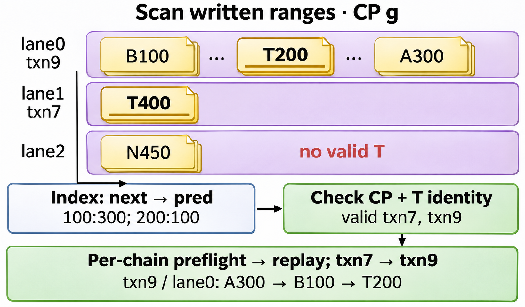
\includegraphics[width=\columnwidth]{./figures/redraw_recovery.pdf}
\caption{Physical scanning and ordered recovery. Only nonterminal NODE next addresses enter the predecessor index. After validating candidate terminals, recovery processes chains in commit-number order by backtracing, forward preflight, and replay. Partial commits without a valid T establish no completion boundary. Addresses and commit numbers are illustrative.}\label{fig:recovery}
\end{figure}

\subsection{Reusing Namespace Commits Completed by Checkpoints}\label{sec:namespace}
Namespace obligations, including parent-directory relationships, can still constrain file-content PACK commits.
Z-ParaPack associates these obligations with completed checkpoints so subsequent synchronization can reuse durable results without repeating a checkpoint for the same obligations.
New namespace changes invalidate the old proof.

A successful checkpoint publishes the proof.
With PACK replay and strict MAIN routing enabled, dirtying directory obligations advances a shared change generation.
A checkpoint snapshots that generation at its start and publishes the committed generation after success.
Synchronization uses the proof only when both generations match and are nonzero.
It also checks that generations have not exhausted their range, checkpointing has no error and remains enabled, and no forced checkpoint request awaits service.

Regular-file and directory synchronization check their respective commit conditions.
For a singly linked, unencrypted regular file, synchronization holds the inode synchronization guard and checks the checkpointed inode node, valid parent number, and shared generation under the inode metadata lock.
It then corrects the in-memory parent information.
Directory synchronization retains DATA writeback waits and checks for dirty state, in-flight writeback, and errors.
A clean directory with a valid proof reuses the completed checkpoint; other cases execute a checkpoint.
Both synchronization paths only read the proof.

\subsection{Implementation and Supported Paths}\label{sec:implementation}
Owners and SIT shards support parallel execution of the commit protocol.
Among owners that can request a file-update lane, synchronization favors the owner with the fewest unreleased application admission tokens.
The count includes queued and executing requests.
Ties favor the file's existing owner hint, while the lane lease still grants append permission.
Owner count, request-lane width, and SIT shard count have separate configurations.

We call the task initiating a DATA writeback batch its producer.
A producer with a valid batch lease can execute allocation callbacks directly, reducing cross-thread delegation.
Admission checks the task, file mapping, filesystem, lane, and generation, and excludes error, teardown, GC, and quota paths.
The callback disables task migration and retains curseg, SIT, and physical-zone locks.
Other cases use the existing local or owner-delegated path, and BIO submission follows existing owner rules.

On overwrite, SIT marks the new block valid and the old block invalid.
The system selects shared protection shards by section number modulo sixteen and acquires relevant shards in a fixed order.
Ordinary local updates take global read-side protection; segment allocation boundaries and global space-state transitions take exclusive protection.
The on-disk SIT layout remains unchanged.

The implementation uses a new format, log-structured (LFS) mode, and strict MAIN routing.
It integrates ordinary buffered writeback, file synchronization, and corresponding NODE, directory, quota, and GC writes.
Format or inode admission rejects unsupported combinations involving encryption, compression, verity, atomic/copy-on-write (COW), or pinned files.
Supported zoned direct-write paths can fall back to buffered writes; workload definitions follow the I/O paths that execute.

\section{Evaluation}\label{sec:evaluation}
\subsection{Experimental Setup and Metrics}\label{sec:setup}
Microbenchmarks examine the scalability of independent synchronous updates; a macrobenchmark tests mixed file operations; applications measure transaction and persistent-publish completion rates.
Mechanism and cost analysis examines changes on synchronization paths, while recovery experiments check commit semantics.
We evaluate the GOOD12.1 implementation of Z-ParaPack.
The fio, FileMicro, and NATS comparisons include F2FS, XFS, Btrfs, ScaleLFS, and Z-LFS.
SQLite and extended Varmail compare against F2FS, Btrfs, ScaleLFS, Z-LFS, DeLFS, MAX, and F2FSJ; OceanBase includes all nine systems.

\begin{table}[t]\centering
\caption{Platform and system configuration.}\label{tab:platform}
\small\setlength{\tabcolsep}{3pt}
\begin{tabularx}{\columnwidth}{@{}P{.19\columnwidth}Y@{}}\toprule
Item & Configuration \\
\midrule
Host & Two Xeon Gold 5218 processors; 32 physical cores, 64 logical CPUs; Linux 7.2.9 \\
Storage & AF3UP44ZTEIG8T0A ZNS SSD; firmware OI1T1129; common 546-zone data region; active/open limits of sixteen each \\
Z-ParaPack & GOOD12.1; fifteen file-update lanes, one maintenance lane; sixteen owners and sixteen SIT shards \\
Native baselines & F2FS, XFS, Btrfs \\
Research baselines & ScaleLFS and Z-LFS: same-kernel ports; DeLFS: local adaptation; MAX and F2FSJ: prototype deployments \\
\bottomrule\end{tabularx}
\end{table}

All systems use the common ZNS region in Table~\ref{tab:platform}.
Z-ParaPack, F2FS, and ScaleLFS place fixed metadata in a 24\,GiB region on a conventional device, with main DATA/NODE on ZNS.
XFS uses a 32\,GiB conventional metadata region and ZNS realtime file data, with \texttt{max\_open\_zones=8}.
Btrfs and Z-LFS use a single ZNS layout.
fio uses logical CPUs 0 through 63.
SQLite clients bind to even-numbered CPUs, with Z-ParaPack owners on non-uniform memory access (NUMA) node~0; other Filebench and application workloads use the default owner configuration.

Z-ParaPack retains ordinary DATA/NODE writes, FLUSH, and the FUA that terminals require.
We use fio 3.28, Filebench 1.4.9.1, NATS Server 2.15.0, and nats.go 1.45.0.
Initialization and preloading precede timing; performance runs disable probes, while allocation counts and path diagnostics use separate runs.
Application baselines include observations across dates under the same implementation, configuration, and workload recipe; comparisons use descriptive statistics.
Table~\ref{tab:workloads} defines operations and completion metrics.
Each result specifies run counts and aggregation.
Asterisks in figures identify local adaptations or ports; daggers identify prototype deployments.
Supplementary Sections~S1 and S2 retain complete Filebench and application results and SQLite latency distributions.

\begin{table}[t]\centering
\caption{Benchmark operations, synchronization semantics, and completion metrics.}\label{tab:workloads}
\small\setlength{\tabcolsep}{3pt}
\begin{tabularx}{\columnwidth}{@{}P{.19\columnwidth}Y@{}}\toprule
Workload & Operations, synchronization, and metric \\
\midrule
FileMicro & Sixteen independent 1\,GiB files; 2\,KiB random writes; WriteRandDsync maps dsync to O\_SYNC. Metric: successful synchronous writes/s. \\
Varmail & One process, sixteen threads; deletes, creates, reads, random appends, and two explicit fsync operations~\cite{r10}. Metric: total flowops/s, including non-write operations. \\
NATS JetStream & Native FileStorage; sixteen streams and publishing connections; \texttt{sync\_interval=always}~\cite{r11}. Metric: successful publishes per second, from a common barrier through the final acknowledgment (ACK). \\
SQLite & Eight databases/64\,KiB or sixteen databases/16\,KiB; each worker updates an independent database, one row per transaction; write-ahead logging (WAL), \texttt{synchronous=FULL}, 1000-page automatic checkpoint threshold. Metrics: transactions/s over the full interval including connection closure; transaction latency. \\
\bottomrule\end{tabularx}
\end{table}

PACK admission checks the inode's dirty DATA page count at synchronization entry.
The limit is sixteen pages for ordinary fio conditions and 1024 pages for 128\,KiB updates and path diagnostics.
Filebench and application benchmarks set the limit to zero, removing this count limit while retaining closure and resource feasibility checks.
Requests exceeding the limit fall back to the original synchronization path.
Reproduction materials retain complete formatting, mount, module-version, and workload recipes.

\subsection{Microbenchmarks: Concurrent Synchronous Updates}\label{sec:micro}
Z-ParaPack's advantage emerges as independent file-update concurrency increases.
fio uses \texttt{psync}, \texttt{pthread}, \texttt{iodepth=1}, and \texttt{direct=0}.
Each thread updates its own file and waits for \texttt{fsync} after every write.
Files total 16\,GiB; timing lasts 600 seconds after prefill and synchronization.
Figure~\ref{fig:scaling}(a, b) covers one through 32 threads with 4\,KiB and 64\,KiB updates, corresponding to one and sixteen DATA pages.
Completion rates include durability of DATA and related NODEs.
Each of the sixteen synchronous-random-write conditions has one run.

\begin{figure*}[t]\centering
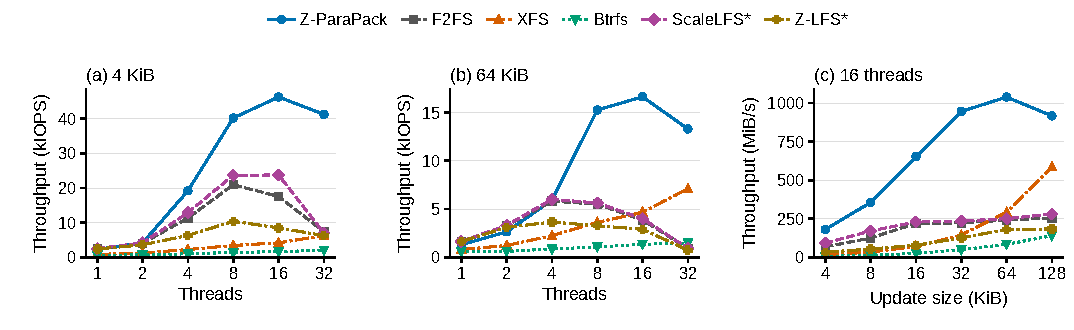
\includegraphics[width=\textwidth]{./figures/compact_fio_scalability.pdf}
\caption{Synchronous random overwrites. (a, b) Concurrency scaling with 4\,KiB and 64\,KiB updates; (c) update-size comparison at sixteen threads.}\label{fig:scaling}
\end{figure*}

At 32 threads, Z-ParaPack reaches 41.27\,kIOPS for 4\,KiB updates, 5.58$\times$ F2FS (7.40\,kIOPS), the fastest baseline under that condition.
For 64\,KiB updates, it reaches 13.30\,kIOPS, 1.87$\times$ the fastest baseline, XFS (7.12\,kIOPS).

Among the concurrency points in Figure~\ref{fig:scaling}, Z-ParaPack exceeds the fastest corresponding baseline from four threads for 4\,KiB and eight threads for 64\,KiB.
At eight threads, 64\,KiB updates already reach 15.26\,kIOPS, 2.71$\times$ the fastest baseline, ScaleLFS.
Thirty-two workers reuse fifteen file-update lanes within the same zone region and active/open limits.
Request count can exceed lane count because completed PACKs return append permission for subsequent updates.

At sixteen threads, Z-ParaPack achieves the highest completed bandwidth for every tested update size: 4, 8, 16, 32, 64, and 128\,KiB.
Its bandwidth reaches 1.56$\times$ to 4.02$\times$ the fastest baseline under each condition.
Figure~\ref{fig:scaling}(c) retains synchronization after every write, covering single-page through 128\,KiB multipage updates.

FileMicro exercises the same problem through O\_SYNC writes.
Sixteen threads issue 2\,KiB synchronous random writes to independent files, with one write operation per WriteRandDsync worker.
Z-ParaPack reaches 1.91$\times$ the successful-write rate of ScaleLFS, the fastest baseline (Figure~\ref{fig:filemicro}).
The comparison runs for 300 seconds, with one independent run per system across six systems.
Bars show run rates.

\begin{figure}[t]\centering
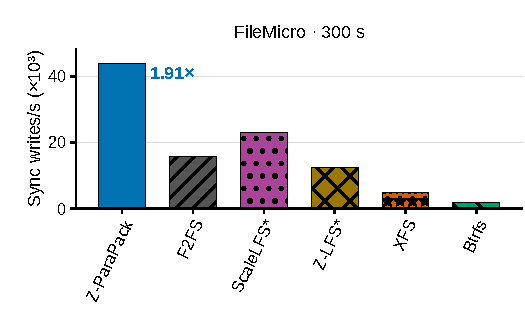
\includegraphics[width=\columnwidth]{./figures/main_filemicro_throughput.pdf}
\caption{FileMicro synchronous random writes. The blue ratio compares against the fastest baseline.}\label{fig:filemicro}
\end{figure}

\subsection{Macrobenchmark: Mixed File Operations}\label{sec:macro}
Extended Varmail combines deletes, creates, reads, appends, and explicit \texttt{fsync} calls into a file-operation stream~\cite{r10}.
Z-ParaPack reaches 101,538.68\,flowops/s, 33.7\% above the fastest baseline, ScaleLFS at 75,955.69\,flowops/s (Figure~\ref{fig:varmail}).
The workload uses 10,000 files, a mean file size of 1\,MiB, mean appends of about 64\,KiB, and a 128\,KiB append upper bound.
Total flowops include non-write operations and measure completed mixed operations.

\begin{figure}[t]\centering
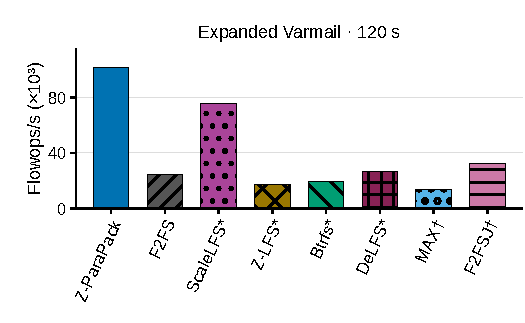
\includegraphics[width=\columnwidth]{./figures/main_varmail_extended.pdf}
\caption{Extended Varmail total flowops/s, including non-write operations. Bars show geometric means of run rates. Asterisks identify local adaptations; daggers identify prototypes.}\label{fig:varmail}
\end{figure}

All eight systems run for 120 seconds.
DeLFS, MAX, and F2FSJ each have two runs; the others each have three.
The mixed workload alternates creation, deletion, and synchronization, extending the single-operation write comparison to filesystem workflows that include namespace changes.

\subsection{Applications: Database Transactions and Persistent Services}\label{sec:applications}
SQLite, NATS, and OceanBase count completed transactions, persistent-publish ACKs, and completed event transactions, respectively.
Controlled clients drive these database and messaging systems to test whether parallel filesystem commits improve application completion rates.

\textbf{SQLite transactions and extreme tail latency.}
Each SQLite worker updates an independent database, modifying one row per transaction.
Table~\ref{tab:workloads} specifies WAL, \texttt{synchronous=FULL}, and automatic checkpoints.
The sixteen-database/16\,KiB configuration reaches 1.94$\times$ its fastest baseline, F2FS; eight databases/64\,KiB reaches 1.37$\times$ its fastest baseline, ScaleLFS (Figure~\ref{fig:sqlite-rate}).
Both configurations run for 120 seconds.
Every system has three runs with sixteen databases.
With eight databases, DeLFS, MAX, and F2FSJ have two runs each, and the others have three.
Bars show geometric means of independent run rates.

\begin{figure}[t]\centering
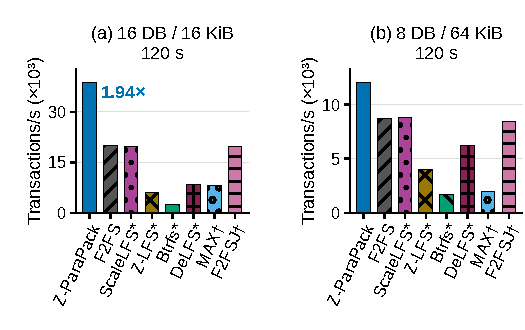
\includegraphics[width=\columnwidth]{./figures/main_sqlite_throughput.pdf}
\caption{SQLite transaction completion rates. (a, b) Sixteen databases/16\,KiB and eight databases/64\,KiB. Blue ratios compare against the fastest baseline in each configuration. Bars show geometric means. Asterisks identify local adaptations; daggers identify prototypes.}\label{fig:sqlite-rate}
\end{figure}

Higher throughput accompanies lower p99.9.
Z-ParaPack achieves the lowest p99.9 among all eight systems in both configurations.
With sixteen databases/16\,KiB, its 13.89\,ms is 73.4\% below Btrfs at 52.14\,ms, the lowest-latency baseline.
With eight databases/64\,KiB, its 10.75\,ms is 23.1\% below ScaleLFS at 13.99\,ms, the lowest-latency baseline.
Throughput and p99.9 comparisons use the fastest and lowest-latency baseline, respectively, within each configuration.

\begin{figure}[t]\centering
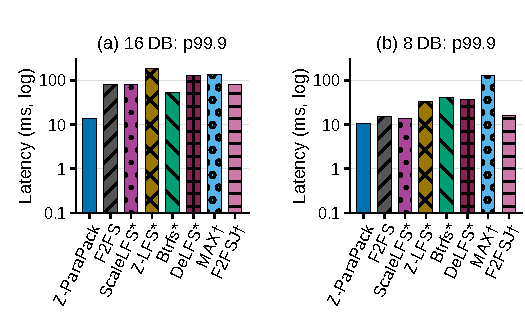
\includegraphics[width=\columnwidth]{./figures/main_sqlite_p999.pdf}
\caption{SQLite p99.9 with (a) sixteen databases/16\,KiB and (b) eight databases/64\,KiB. Millisecond axes use logarithmic scales with a 0.1\,ms bar baseline. Bars show geometric means of run-level quantiles. Asterisks identify local adaptations; daggers identify prototypes.}\label{fig:sqlite-tail}
\end{figure}

Transaction latency includes transaction start, update, commit, and lock-conflict retries before success.
For each run, we merge worker histograms in integer microseconds and compute nearest-rank p99.9.
We then take the geometric mean of these run-level quantiles.
Transaction rates cover the complete run interval, including connection closure.

\textbf{NATS persistent publishing.}
NATS JetStream publishes persistently across sixteen streams.
Z-ParaPack reaches 1.88$\times$ the successful-publish rate of ScaleLFS, the fastest baseline (Figure~\ref{fig:nats}).
Messages contain JSON from real AWS CloudWatch records~\cite{r12}, with sixteen fixed publishing connections and native FileStorage using \texttt{sync\_interval=always}~\cite{r11}.
Completion rates span the common publishing barrier through the final ACK, including waits for persistence confirmation.
The comparison lasts 300 seconds, with one independent run per system across six systems.

\begin{figure}[t]\centering
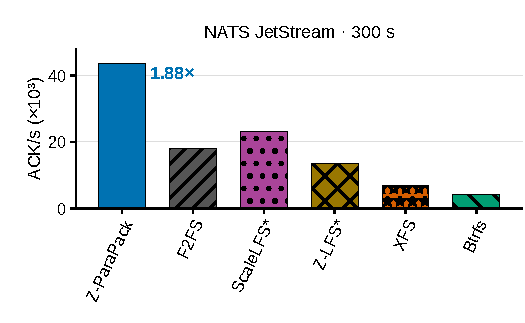
\includegraphics[width=\columnwidth]{./figures/main_nats_throughput.pdf}
\caption{NATS JetStream successful-publish rates. The blue ratio compares against the fastest baseline.}\label{fig:nats}
\end{figure}

\textbf{OceanBase multi-tenant event commits.}
With 128 OceanBase clients, Z-ParaPack increases mean throughput by 69.6\% over F2FS controls from the same cohort.
Throughput exceeds ScaleLFS and DeLFS by 66.0\% and 38.7\%, respectively.
Figure~\ref{fig:oceanbase} reports absolute event completion rates for all nine systems.

The workload uses two colocated, independent, single-replica OceanBase instances, with sixteen tenants and 128 closed-loop clients in total.
It preserves order within each repository while replaying 865,942 issue and pull-request events from the complete UTC day of January 6, 2025, in GH Archive~\cite{r15}.
Each event executes one autocommit transaction that retains the full JSON and reconstructs the entity's latest state.
The instances together use 32 logical service CPUs and 96\,GiB of configured memory; the database handles underlying log synchronization.

Completion rate divides all input events by wall-clock time from common client release until all clients exit.
Each baseline has two independent fresh-filesystem runs.
Comparisons use the corresponding cohort's GOOD controls and arithmetic means of run-level metrics; the GOOD bar pools eight observations.
Supplementary Section~S3 retains complete cohort results, latency distributions, and protocols.

\begin{figure}[t]\centering
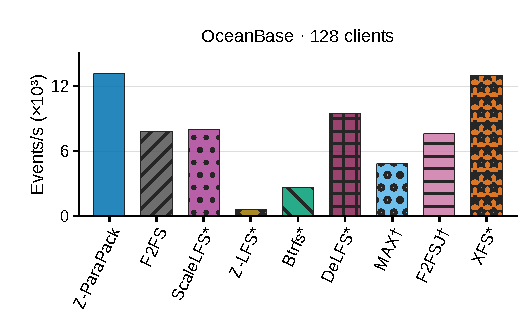
\includegraphics[width=\columnwidth]{./figures/main_oceanbase_throughput.pdf}
\caption{OceanBase full-JSON event completion rates. Bars show arithmetic means. Z-ParaPack pools eight observations, with two per baseline; text comparisons use matching cohort controls. Asterisks identify local adaptations; daggers identify prototypes.}\label{fig:oceanbase}
\end{figure}

\subsection{Mechanisms and Costs}\label{sec:cost}
\textbf{Shared-allocation intervals.}
F2FS shared-allocation intervals grow with concurrency; Z-ParaPack separates independent updates' append state across lanes.
In the request-correlated diagnostics of Figure~\ref{fig:breakdown}, increasing threads from eight to 32 raises F2FS combined DATA/NODE curseg time from 1.197 to 38.369\,ms.
The full sampled \texttt{fsync} grows from 2.716 to 40.845\,ms.
At eight, sixteen, and 32 threads, Z-ParaPack combined curseg time stays below 0.18\,ms, and the full sampled call stays below 1.4\,ms.

\begin{figure*}[t]\centering
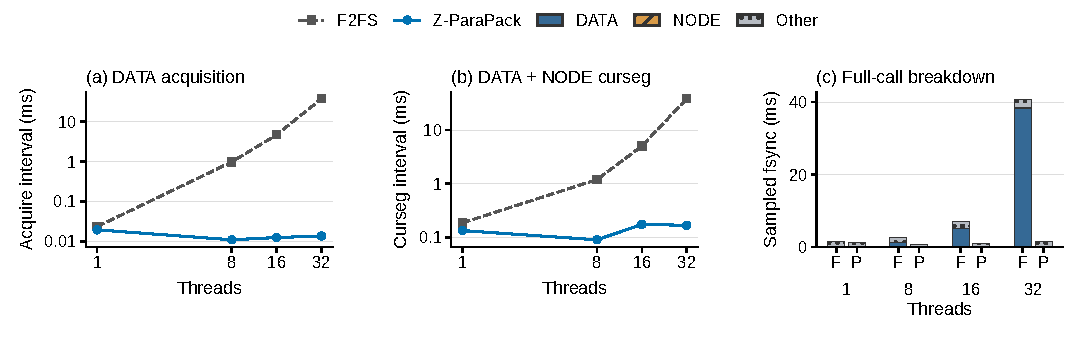
\includegraphics[width=\textwidth]{./figures/compact_fsync_breakdown.pdf}
\caption{Allocation intervals and full sampled fsync calls. (a) DATA curseg acquisition; (b) combined DATA/NODE curseg time; (c) full-call breakdown, with F/P denoting F2FS/Z-ParaPack. Lines and bars show sample means within independent diagnostic runs. The first two panels use logarithmic millisecond axes.}\label{fig:breakdown}
\end{figure*}

At 32 threads, DATA curseg acquisition falls from F2FS's 37.785\,ms to Z-ParaPack's 13.544\,$\mu$s.
Combined DATA/NODE curseg time falls from 38.369 to 0.168\,ms, occupying 12.2\% of Z-ParaPack's full sampled call.
The full call takes 1.378\,ms, 96.6\% shorter than F2FS.
These changes accord with the separated append state in Sections~\ref{sec:overview} through~\ref{sec:lease} and address the shared entry points in Figure~\ref{fig:motivation}.

Diagnostics use separate runs.
Allocation counts in Figure~\ref{fig:motivation}(b) use 64\,KiB writes followed by \texttt{fsync}, one/two/four threads, 16\,GiB per thread, and 60-second runs.
Figures~\ref{fig:motivation}(c) and~\ref{fig:breakdown} use one/eight/sixteen/32 threads, 256\,MiB per thread, and 30-second runs, sampling every 64th \texttt{fsync} per inode.
Each condition has one run, and both diagnostic protocols start after prefill and synchronization.
Path sampling covers the complete \texttt{fsync} and partitions DATA/NODE curseg acquisition and hold time into disjoint intervals, giving \texttt{balance} priority and assigning remaining time to Other.
Acquisition includes execution, queuing, and scheduling.
Z-ParaPack correlates local and delegated allocation callbacks for each request and classifies them by logical DATA/NODE type.

\textbf{CPU cost per write and synchronization tail latency.}
Figure~\ref{fig:cpu} uses the same 600-second performance runs as Figure~\ref{fig:scaling}(a, b), covering all six systems and conditions.
fio mean \texttt{fsync} latency weights each worker by its call count; tail latency takes the maximum worker p99.
CPU cost per completed write accumulates busy time across all logical CPUs over the full fio invocation, including filesystem threads, startup, and teardown.

At 4\,KiB and 32 threads, Z-ParaPack uses 182.64\,$\mu$s/write and has a maximum worker \texttt{fsync} p99 of 1.352\,ms.
F2FS, the fastest throughput baseline under that condition, uses 423.56\,$\mu$s/write with a 7.045\,ms tail.
At 64\,KiB and 32 threads, Z-ParaPack uses 635.69\,$\mu$s/write with a 2.966\,ms tail, compared with 815.50\,$\mu$s/write and 6.390\,ms for XFS.
As concurrent completion increases, host CPU time per completed write and synchronization tail latency also decrease.

\begin{figure*}[t]\centering
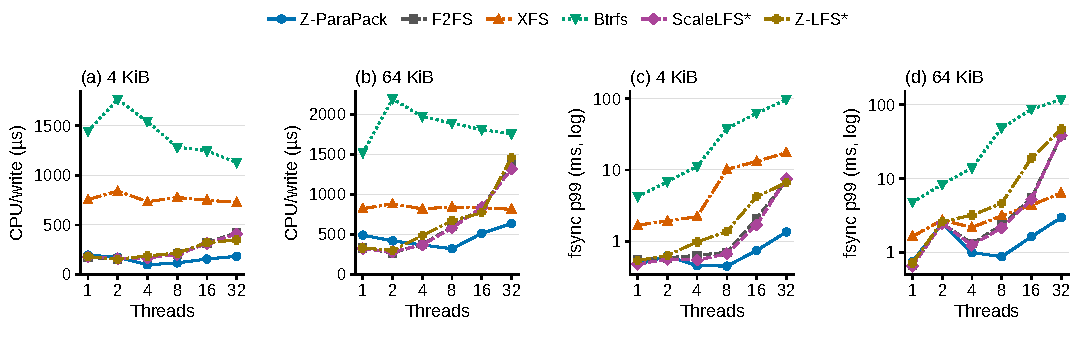
\includegraphics[width=\textwidth]{./figures/compact_fio_cost_tail.pdf}
\caption{Host CPU cost per completed write and maximum worker fsync p99. (a, b) CPU cost for 4\,KiB and 64\,KiB updates; (c, d) corresponding tail latency on logarithmic axes.}\label{fig:cpu}
\end{figure*}

\textbf{Namespace-commit reuse.}
The proof in Section~\ref{sec:namespace} lets subsequent synchronization reuse a completed checkpoint.
Enabling this mechanism within the same GOOD12.1 module increases throughput by 5.55\% and 5.00\% across two OceanBase controls.
It reduces p99 by 14.96\% and 13.41\%, respectively (Table~\ref{tab:namespace}).
These within-module controls use one instance, sixteen tenants, and four clients per tenant, totaling 64 clients.
Each state has one independent run under each order, OFF-to-ON and ON-to-OFF.
We analyze these separately from the 128-client cross-system comparison in Section~\ref{sec:applications}.
OceanBase merges transaction histograms within each run before computing tail latency.

\begin{table}[t]\centering
\caption{Within-module namespace-commit reuse with 64 clients.}\label{tab:namespace}
\small\setlength{\tabcolsep}{3pt}
\begin{tabular}{@{}llrr@{}}\toprule
Run order & State & Events/s & p99 (ms) \\
\midrule
OFF to ON & OFF & 11,031.04 & 23.521 \\
OFF to ON & ON & 11,642.76 & 20.002 \\
ON to OFF & OFF & 11,102.28 & 22.284 \\
ON to OFF & ON & 11,657.33 & 19.295 \\
\bottomrule\end{tabular}
\end{table}

The ON state reuses parent-number and directory-synchronization proofs; corresponding reuse counts remain zero in the OFF state.

\subsection{Commit Contents and Logical Recovery}\label{sec:logical}
Confirmed PACK contents remain recoverable after interruptions of subsequent commits.
Table~\ref{tab:recovery} organizes logical interruption scenarios around mapping closures, completion boundaries, and generation-scoped recovery in Sections~\ref{sec:closure}, \ref{sec:terminal}, and~\ref{sec:recovery}.
Z-ParaPack recovers complete files after successful \texttt{fsync} ACKs and continues with next-generation writes after restoring checkpoint state.
Experiments use the same GOOD12.1 module and Linux 7.2.9 virtual machines with memory-backed devices.
Predetermined complete file bytes provide the content oracle.
NOSYNC denotes interruption without generating a new checkpoint.

\begin{table}[t]\centering
\caption{GOOD12.1 content and logical recovery tests.}\label{tab:recovery}
\small\setlength{\tabcolsep}{3pt}
\begin{tabularx}{\columnwidth}{@{}P{.25\columnwidth}Y@{}}\toprule
Test group & Interruption scenario and content check \\
\midrule
Confirmed commits & Eight ACKs; recover after NOSYNC logical interruption and check all 32\,MiB byte for byte. \\
Incomplete terminal & Eight previous ACKs; inject a timeout before terminal submission, causing fsync to return EIO; interrupt the partial commit and recover the confirmed 32\,MiB. \\
Asynchronous mappings & Write DATA asynchronously, then synchronize pending mappings; eight ACKs; recover and check 32\,MiB after NOSYNC interruption. \\
Checkpoint and subsequent writes & Sixteen 192\,KiB files; checkpoint, then NOSYNC interruption; recover all bytes, write the next generation, and remount read-only; reclaim a checkpointed open-but-unlinked inode. \\
\bottomrule\end{tabularx}
\end{table}

The terminal distinguishes completed updates from partial commits.
All 32\,MiB confirmed by eight ACKs recover byte for byte after interruption.
Injecting a timeout before a subsequent terminal submission causes \texttt{fsync} to return EIO without damaging earlier acknowledged contents.
The asynchronous-writeback scenario first writes DATA, then synchronizes pending mappings, and recovers all 32\,MiB.
This tests the cross-lease obligation in Section~\ref{sec:joint}: mappings still require confirmation after DATA dirty flags clear.

Checkpoint recovery retains committed state and permits subsequent updates.
All sixteen 192\,KiB files match after recovery; read-only remount verifies next-generation writes, and recovery reclaims the checkpointed open-but-unlinked inode.
Across all four groups, both checkpoint packs retain identical complete bytes throughout the interruption window.
Post-remount checks inspect structure without repair.
Table~\ref{tab:recovery} tests logical interruptions on memory-backed devices and excludes physical power cuts.
Real-SSD performance runs use normal unmount/remount and content verification.

\section{Related Work}\label{sec:related}
\textbf{Parallel logs and decentralized metadata.}
Max dynamically assigns complete file operations to log partitions.
Each partition contains temperature-classified DATA and inode logs, with recovery merging through global inode versions~\cite{r2}.
DeLFS decentralizes resource and lock ownership and separates critical work from deferrable work~\cite{r4}.
Z-ParaPack gathers current writeback and mapping obligations from earlier writeback into a PACK.
Its closure spans lane leases, while the current selected NODEs and terminal confirm completion.
This organization of parallel appends also specifies the contents that file synchronization must commit.

\textbf{ZNS logs and resource management.}
Z-LFS uses append-only metadata, temperature-based speculative log-stream management, and conflict-aware allocation to exploit small zones~\cite{r5}.
Its 2026 journal extension uses dedicated per-stream writers for parallel writeback~\cite{r17}.
Our comparison uses a port of the ATC-version public source.
ScaleLFS scales reclamation with GC-specific streams and local coordination~\cite{r8}; eZNS manages zone resources and I/O admission at the interface~\cite{r9}.
Z-ParaPack separates returnable lane append permission from persistent physical-zone accounting.
It reuses file-update lanes within common active/open limits and reserves append state for maintenance writes.

\textbf{Synchronization and recovery.}
F2FS node chains, fsync/dentry marks, and checkpoints provide the original recovery foundation~\cite{r1}.
ScaleZNFS uses multihead DATA logs, per-log scheduling, ZNS-driven node ordering, and split fsync-node wait lists.
Each NODE type still uses one log and retains F2FS recovery~\cite{r3}.
F2FSJ collects metadata changes in in-memory per-inode log lists, aggregates them into an on-disk epoch journal, and commits and applies the journal~\cite{r7}.
Ma et al. parallelize DATA and dnode writeback~\cite{r6}.
Z-ParaPack further distributes related NODEs across file-update lanes and confirms completion through the current PACK's terminal.
It recovers node chains and commit order within checkpoint generations, giving completion confirmation and distributed-node recovery the same PACK boundary.

\section{Conclusion}\label{sec:conclusion}
Independent file updates need independent append allocation and durable completion confirmation.
Z-ParaPack gathers current writeback and cross-lease mapping obligations into PACKs and distributes DATA/NODE append state through reusable lanes.
The terminal and checkpoint-scoped node chains define completion and recovery boundaries.
This organization increases concurrent durable-update completion within finite zone limits.
At 4\,KiB and 32 threads, synchronous random writes reach 5.58$\times$ the fastest baseline under the same condition.
With sixteen SQLite databases, transaction completion reaches 1.94$\times$ the fastest baseline, while p99.9 falls 73.4\% below the lowest-latency baseline.
Mixed file operations, messaging, and multi-tenant databases also benefit.
Allocation-path and CPU-cost analyses explain the changes in synchronization overhead at high concurrency.

\section*{Acknowledgments}
OpenAI Codex assisted experiment automation, evidence organization, drafting, and revision during manuscript preparation~\cite{r16}.
% Keep the bibliography heading with its entries in the final right column.
%\newpage
%\begin{thebibliography}{17}
\bibitem{r1} Changman Lee, Dongho Sim, Jooyoung Hwang, Sangyeun Cho. F2FS: A New File System for Flash Storage. FAST 2015, pp. 273-286. \url{https://www.usenix.org/conference/fast15/technical-sessions/presentation/lee}
\bibitem{r2} Xiaojian Liao, Youyou Lu, Erci Xu, Jiwu Shu. Max: A Multicore-Accelerated File System for Flash Storage. USENIX ATC 2021, pp. 877-891. \url{https://www.usenix.org/conference/atc21/presentation/liao}
\bibitem{r3} Haichuan Hu, Jintong Zhang, Miaosong Zhang, Yekang Zhan, Nan Zhang, Jianxi Chen, Dan Feng. Zoned Namespace is a Double-edged Sword: Rethinking the Impact of the ZNS Interface on File System Scalability. ACM Transactions on Storage, 2026. \url{https://doi.org/10.1145/3816706}
\bibitem{r4} Taehwan Ahn, Chanhyeong Yu, Sangjin Lee, Yongseok Son. DeLFS: A Decentralized Log-Structured File System for Manycores. OSDI 2026, pp. 793-807. \url{https://www.usenix.org/conference/osdi26/presentation/ahn}
\bibitem{r5} Inhwi Hwang, Sangjin Lee, Sunggon Kim, Hyeonsang Eom, Yongseok Son. Z-LFS: A Zoned Namespace-tailored Log-structured File System for Commodity Small-zone ZNS SSDs. USENIX ATC 2025, pp. 547-562. \url{https://www.usenix.org/conference/atc25/presentation/hwang}
\bibitem{r6} Mengyang Ma, Yumiao Zhao, Yunpeng Song, Yi Zhang, Shouzhen Gu. Improving F2FS fsync() Latency Through Parallelizing Dnode and Data Page Writeback. NAS 2024, pp. 1-8. \url{https://doi.org/10.1109/NAS63802.2024.10781365}
\bibitem{r7} Yaotian Cui, Zhiqi Wang, Renhai Chen, Zili Shao. Decentralized, Epoch-based F2FS Journaling with Fine-grained Crash Recovery. OSDI 2025, pp. 879-895. \url{https://www.usenix.org/conference/osdi25/presentation/cui}
\bibitem{r8} Jin Yong Ha, Sangjin Lee, Hyeonsang Eom, Yongseok Son. ScaleLFS: A Log-Structured File System with Scalable Garbage Collection for Commodity SSDs. FAST 2025, pp. 53-67. \url{https://www.usenix.org/conference/fast25/presentation/ha}
\bibitem{r9} Jaehong Min, Chenxingyu Zhao, Ming Liu, Arvind Krishnamurthy. eZNS: An Elastic Zoned Namespace for Commodity ZNS SSDs. OSDI 2023, pp. 461-477. \url{https://www.usenix.org/conference/osdi23/presentation/min}
\bibitem{r10} Filebench Project. Filebench workload definitions, source commit 22620e602cbbebad90c0bd041896ebccf70dbf5f; evaluated runtime 1.4.9.1. \url{https://github.com/filebench/filebench/tree/22620e602cbbebad90c0bd041896ebccf70dbf5f/workloads}
\bibitem{r11} NATS Project. JetStream sync\_interval configuration and FileStorage, NATS Server 2.15.0. \url{https://docs.nats.io/reference/config/jetstream/sync_interval/}
\bibitem{r12} Numenta. Numenta Anomaly Benchmark: realAWSCloudwatch data. \url{https://github.com/numenta/NAB/tree/master/data/realAWSCloudwatch}
\bibitem{r13} ScaleLFS Authors. ScaleLFS public source code, ScaleLFS/segment.c, segment.h and data.c; master content snapshot checked 2026-10-14. \url{https://github.com/syslab-CAU/ScaleLFS/tree/master/ScaleLFS}
\bibitem{r14} Z-LFS Authors. Z-LFS public source code, commit d1f8ea8f358e43352055237353ab37f01dfa801a, linux-5.17.4/fs/f2fs/segment.c, segment.h and data.c. \url{https://github.com/Z-LFS/Z-LFS/tree/d1f8ea8f358e43352055237353ab37f01dfa801a/linux-5.17.4/fs/f2fs}
\bibitem{r15} GH Archive Project. GH Archive: public GitHub event archives. Dataset: January 6, 2025 UTC, hourly JSON archives. \url{https://www.gharchive.org/}
\bibitem{r16} OpenAI. Codex. AI coding agent. Accessed November 14, 2026. \url{https://openai.com/codex/}
\bibitem{r17} Inhwi Hwang, Sangjin Lee, Sunggon Kim, Hyeonsang Eom, Yongseok Son. Design and implementation of zoned namespace-tailored log-structured file system for commodity ZNS SSDs. Future Generation Computer Systems, vol. 183, article 108563, Oct. 2026. \url{https://doi.org/10.1016/j.future.2026.108563}
\end{thebibliography}

\bibliographystyle{IEEEtran}
\bibliography{refer}
\end{document}
